\chapter{Background to the project}

\section{Problem Description}

Improvements of high density power storage, integrated miniature actuators and
sensors, facilitate the development of \MAV and new areas of research for
unmanned and autonomous flying systems \citebib[p.1 Introduction]{BourMurSie04}.
 This new area of interest brought also a new area of problems.
 One of these is the fact that the pilot of the aerial vehicle does not exist,
 because the \UAV flights autonomous or the pilot observes and controls the \UAV via
 remote control. In both cases it is necessary that the \UAV system can detect
 its absolute position, to provide the pilot a better quality of control or
 furthermore to manoeuvre autonomous. The following articles also describe this
 problem with different views and approaches 
\citebib[p.2 Localization and path planning]{GrzGriBur09}
\citebib[p.1 High precision aircraft positioning]{WenMasZel10} 
\citebib[p.2 Teleoperated Robot Control]{BluHolLinMolSurViaTre08}.


This necessity of location determination requires measurement unit, which
provides the detection of the movements in the given \DOF. Because of low-cost
and low-complexity reasons, the most popular components which are used to reach
a nearly satisfactorily level of flight stabilization are inertial sensors.
These sensors combined together called \IMU and have the ability to detect the
acceleration of translational or rotational movements.
\newpage Furthermore a control
system can be used in a closed loop together with the \IMU and can correct
theoretically nearly every disturbance in a continual system 
\citebib[p.p.45-64 System Control]{Bou07}
\citebib[p.p.49-51 Control Strategy]{CasLozAle05}.
The limitation of resolution of the sensors and the necessity of integrating the
acceleration values for position and velocity determination, have in real systems
a big impact in aspects of error propagation and detection of smoothly movements
 \citebib[p.5 Low-acceleration Drift]{Tip08}.
For a better appreciation of the movements, the following figure visualizes the
influence of the thrust in relation to the movements in the \DOF s. Thereby the
 values of  \ensuremath{\omega} \lbrack rad/sec \rbrack represents the least
needed speed of rotation, for creating the required thrust for the hovering
state. This state can be described as a state, in which forces in the x- and
y-axis equals zero and the uplift force in direction of the z-axis has the
same absolute value as the gravitational force. The value of 
\ensuremath{\Delta}\ensuremath{\omega} characterizes the purposed deviation of the required force
in hovering state and is used for navigation of the quadrocopter.


\begin{figure}[!htbp]
	\centering
		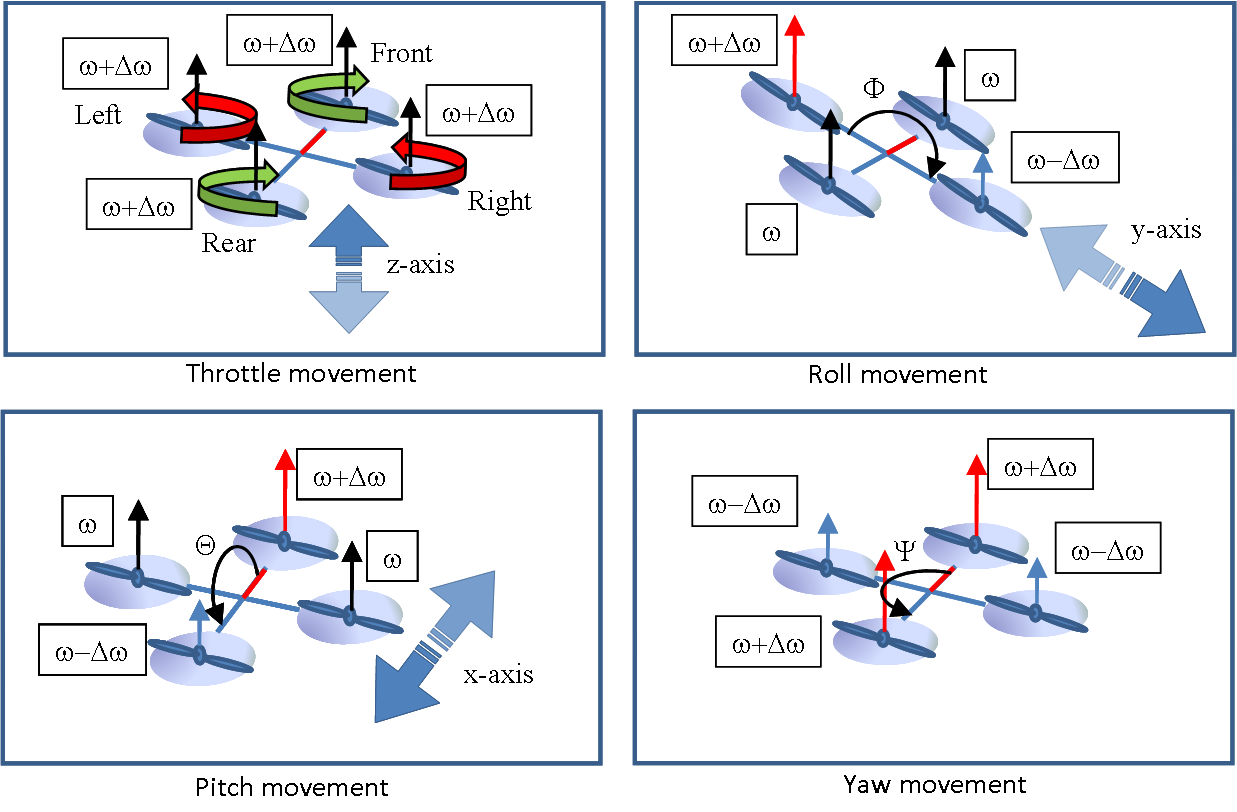
\includegraphics[width=0.75\textwidth]{graphic/QuadrotoDOF.png}
	\caption{Degrees of Freedom of a quadrocopter}
	\label{fig:quadrotoDOF}
\end{figure}

\newpage
To keep the equilibrium of rotational kinematics and to prevent self-rotation,
the motor direction of rotation equals crosswise. The quadrocopter has six \DOF
which can be distinguished as angular and translational movements.
Translational movements can be executed in x-, y- and z- axis. Accelerating all rotors with
the same thrust \ensuremath{\omega} to the value of
\ensuremath{\Delta}\ensuremath{\omega}  will affect a movement in z-direction.
Movements to the negative direction of the z-axis are possible, if the thrust of
the four rotors is smaller as the gravitational force of the aerial vehicle.

 The roll movements can be described as a change of the angle around the x-axis.
Thereby the left and right rotors execute a force difference by slowing down
the one and simultaneous increasing the other thrust with
\ensuremath{\Delta}\ensuremath{\omega}. Related to the thrust difference and angular
 movement, the aerial vehicle creates a force to the y-axis. Equivalent to roll,
 the pitch movement is executed with a change of the angle around the y-axis.
 Also the pitch movement creates a translational
movement across the x-axis. Pitch and roll can only reach a stable angular state
and accelerate to the x- or y-axis, if the value of
\ensuremath{\Delta}\ensuremath{\omega} 
is the same at the diagonal rotors. Otherwise, the quadrocopter would pure rotate
across the corresponding axis.

 The yaw movement is a rotation around the z-axis.
This angular movement results in combination of pairwise different thrusts and
takes as long as the thrusts are different
 \citebib[p.p.8-11 Quadrotor model and system]{CasLozAle05}.
\newline
Synthesizing the weaknesses of \MEMS like noise or the limited resolution,
together with the characteristics of the kinematics of the quadrocopter shows
the problems which come up in case of \MAV control with a \IMU with \MEMS. As
mentioned smoothly accelerations could be a drawback for the control system,
because this kind of accelerations gets lost in the sensor noise.
\newpage
 Regarding the kinematics of the quadrocopter, we have seen that translational
 movements can only be reached with angular movements across the x- and y-axis of with
increasing or decreasing the thrust on every rotor in the z-axis. Imprecise
noisy sensors would affect a wrong thrust regulation at the actuators. Thereby
it is highly improbable, that all four rotors affected by the noise equal and
accelerate in the z-axis. More probable as a uncontrollable acceleration in the
direction of the z-axis, is that pairwise two rotors have the some drift and
create so an unexpected yaw rotation. Finally the most probable will be a
wrong thrust regulation at one rotor, but for a short time interval. So the most
likely error drifts will exist at the x- and y-axis. So the hovering state will
be nearly impossible to reach just with \MEMS acceleration sensors, because the
x- and y- movements have to be zero. 

The following figure \ref{fig:ImpactOfNoise} shows the described problem area
 of \MEMS sensors in the concrete case of the sensors which are mounted at the
quadrocopter \CCU of the \HSE. The mechanical characteristics of the translational acceleration sensor
\citebib [pp.37-39 Typical performance characteristics]{ST05_1}
were simulated under consideration of the change of the position of the
quadrocopter and the applied acceleration.\newpage We can see, that
accelerations which are small enough, get lost in the sensor noise and are invisible for the
quadrocopter. Furthermore the quadrocopter reacts in t=12 if the
acceleration transcends the threshold value of the sensor noise.


\begin{figure}[!htbp]
	\centering
		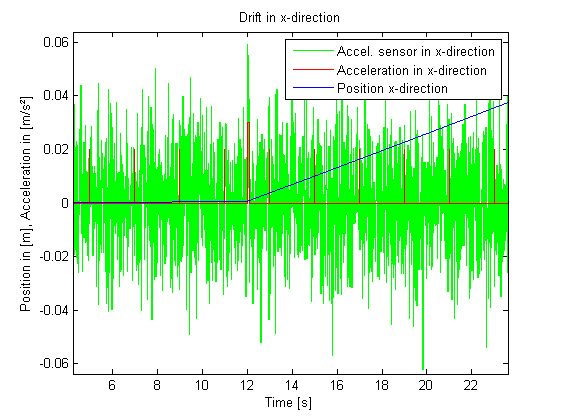
\includegraphics[width=0.75\textwidth]{graphic/ImpactOfNoise.png}
	\caption{The impact of sensor noise}
	\label{fig:ImpactOfNoise}
\end{figure}
